\documentclass{report}
\usepackage{fancyhdr} % Required for custom headers
\usepackage{lastpage} % Required to determine the last page for the footer
\usepackage{extramarks} % Required for headers and footers
\usepackage{graphicx} % Required to insert images
%\usepackage{lipsum} % Used for inserting dummy 'Lorem ipsum' text into the template
\usepackage{amsmath}
\usepackage{float}
\usepackage{graphicx} 
%\usepackage{amsfont}
%\usepackage{amssymb}

\usepackage{multicol}
% Margins
\topmargin=-0.5in
\evensidemargin=0in
\oddsidemargin=-0.5in
\textwidth=7.5in
\textheight=9.0in
\headsep=0.25in 


\pagestyle{fancy}

%\rhead{\textbf{Marshall's Recipes}} % Top right header
%\lhead{\textbf{Curry Stir Fry}}
%\chead{ }
%\title{Curry Stir Fry}

\begin{document}
%\vspace{8mm}
%\textbf{PRELIMINARIES:}


\bigskip

\bigskip

\begin{multicols}{2}
\textbf{Ingredients}
\begin{itemize}
\item 1 cups flour \quad (456 kCal / 14 gP / 1 gF / 96 gC)
\item $\frac{3}{4}$ cup melted butter (1224 kCal / 0 gP / 144 gF / 0 gC)
\item 2 eggs (room temperature)  \quad \newline (156 kCal / 12 gP / 10 gF / 2 gC)
\item 1 cup white sugar (774 kCal/ 0 gP/ 0 gF/ 200 gC)
\item $\frac{3}{4}$ lb. cranberries \quad (157 kCal / 1 gP / 0 gF / 41 gC)
\item $\frac{1}{2}$ cup sliced almonds \quad \newline(240 kCal / 9 gP / 21 gF / 9 gC)
\item 1 teaspoon almond extract 




\end{itemize}


\columnbreak
\textbf{Procedure:}
\medskip


\begin{enumerate}
\item Preheat oven to 325 degrees and grease a pie pan (or tart pan if you have it)


\medskip
\item In a medium bowl, combine $\frac{1}{2}$ cup of sugar, almonds, and cranberries. Transfer to greased pan.  
\medskip

\item In the empty bowl, beat the eggs, butter, almond extract, and remaining sugar until blended. Gradually add flour until mixture thickens (it will be quite thick). Spread evenly over sugared berries. 
\newline 

 \item Bake at 325 degrees for 40-45 minutes or until a toothpick inserted in the center comes out clean. Cool in pan or on a wire rack. If desired, dust with powdered sugar or serve with whipped cream. 
\end{enumerate}
\begin{table}[H]
  \begin{center}
    \caption{Macro totals}
    \label{tab:table1}
    \begin{tabular}{c|c|c|c} % <-- Alignments: 1st column left, 2nd middle and 3rd right, with vertical lines in between
      \textbf{Calories} & \textbf{Protein} & \textbf{Fat} & \textbf{Carbs}\\
      \hline
      3,077 kCal & 36 g & 176 g & 348 g\\
    \end{tabular}
  \end{center}
\end{table}
\end{multicols}



%\begin{center}
%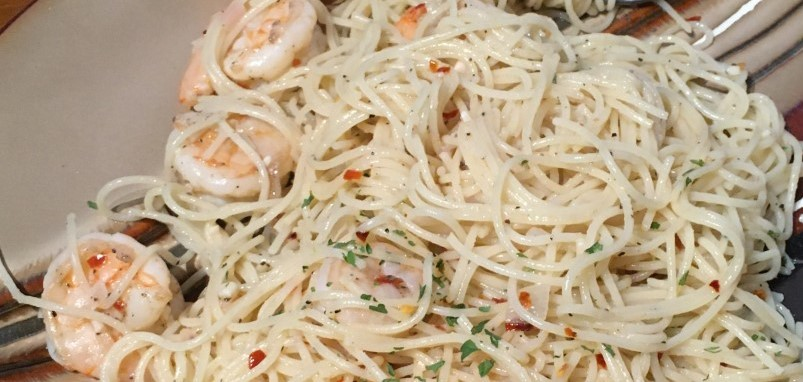
\includegraphics[scale=0.65]{Pasta/Shrimp Scampi/Shrimp Scampi.jpg}
%\end{center}


\end{document}